\documentclass[aspectratio=169]{beamer}

% Shared Beamer settings for Applied Machine Learning lectures (UPES).
% Keep this file free of \documentclass to allow reuse via \input.

% Allow lecture sources to use shared theme/assets without copying them into each lecture folder.
% NOTE: These paths are relative to `Unit-xx/Lecture-yy/latex/` (and `Lab/Experiment-xx/latex/`).
\makeatletter
\def\input@path{{../../../_shared/}{../../../_shared/UPES-Beamer-Theme/}}
\makeatother

\usetheme{UPES}
\setbeamertemplate{navigation symbols}{}

\usepackage{amsmath}
\usepackage{amssymb}
\usepackage{booktabs}
\usepackage{graphicx}
\usepackage{hyperref}
\usepackage{xcolor}
\usepackage{listings}

% Code listings (Python-oriented for this subject).
\lstset{
  language=Python,
  basicstyle=\ttfamily\small,
  keywordstyle=\color{blue},
  commentstyle=\color{gray},
  stringstyle=\color{teal},
  showstringspaces=false,
  columns=fullflexible,
  breaklines=true
}

\usepackage{tikz}
\usetikzlibrary{arrows.meta,positioning,shapes.geometric,calc,fit,backgrounds}

% Per-slide source line (references shown on the slide itself).
\newcommand{\slidesources}[1]{%
  \vfill
  {\tiny\color{gray}\raggedright\sloppy\parbox{\linewidth}{Sources: #1}\par}%
}

% Unit-wise source strings for this subject (used by slides/notes).
% Path is relative to the lecture `latex/` folder (the compilation CWD).
% Source strings for Applied Machine Learning (CSAI2017P) — used by slides + notes.
% Prescribed texts and reference books are taken from the course syllabus.
% Support texts are the author-hosted open-access editions:
%   statlearning.com            (ISL with Python)
%   probml.github.io/pml-book   (Murphy, Probabilistic Machine Learning)
%   d2l.ai                      (Dive into Deep Learning)
%   mml-book.github.io          (Mathematics for Machine Learning)

\newcommand{\AMLRepoURL}{https://github.com/tali7c/Applied-Machine-Learning}

% --- prescribed -------------------------------------------------------------
\newcommand{\AMLPrescribed}{%
M\"uller and Guido, \textit{Introduction to Machine Learning with Python}, O'Reilly, 2016.;%
Bishop, \textit{Pattern Recognition and Machine Learning}, Springer, 2006.;%
Murphy, \textit{Machine Learning: A Probabilistic Perspective}, MIT Press, 2012.;%
Han, Kamber and Pei, \textit{Data Mining: Concepts and Techniques} (3e), Morgan Kaufmann, 2012.%
}

% --- unit-wise ---------------------------------------------------------------
\newcommand{\AMLUnitISources}{%
M\"uller and Guido, \textit{Introduction to Machine Learning with Python}, Ch. 1.;%
Bishop, \textit{Pattern Recognition and Machine Learning}, Ch. 1.;%
Murphy, \textit{Probabilistic Machine Learning: An Introduction}, MIT Press, 2022, Ch. 1.;%
Mitchell, \textit{Machine Learning}, McGraw Hill, 1997, Ch. 1.;%
Scikit-learn documentation, accessed 2026-08-04.%
}

\newcommand{\AMLUnitIISources}{%
Bishop, \textit{Pattern Recognition and Machine Learning}, \S1.5, \S4.3, \S7.1.;%
Zhang, Lipton, Li and Smola, \textit{Dive into Deep Learning}, \S3.4.;%
Shalev-Shwartz and Ben-David, \textit{Understanding Machine Learning}, Ch. 15.;%
Murphy, \textit{Probabilistic Machine Learning: An Introduction}, Ch. 5.%
}

\newcommand{\AMLUnitIIISources}{%
Zhang, Lipton, Li and Smola, \textit{Dive into Deep Learning}, Ch. 12 (Optimization Algorithms).;%
Deisenroth, Faisal and Ong, \textit{Mathematics for Machine Learning}, Ch. 7.;%
Kingma and Ba, ``Adam: A Method for Stochastic Optimization,'' ICLR 2015.;%
Ruder, ``An overview of gradient descent optimization algorithms,'' arXiv:1609.04747, 2016.%
}

\newcommand{\AMLUnitIVSources}{%
Han, Kamber and Pei, \textit{Data Mining: Concepts and Techniques} (3e), Ch. 3.;%
M\"uller and Guido, \textit{Introduction to Machine Learning with Python}, Ch. 3--4.;%
James, Witten, Hastie, Tibshirani and Taylor, \textit{An Introduction to Statistical Learning with Python}, Ch. 5--6, 12.;%
Scikit-learn documentation (preprocessing, model selection), accessed 2026-08-04.%
}

\newcommand{\AMLUnitVSources}{%
James et al., \textit{An Introduction to Statistical Learning with Python}, Ch. 3--6.;%
Bishop, \textit{Pattern Recognition and Machine Learning}, Ch. 3.;%
Deisenroth, Faisal and Ong, \textit{Mathematics for Machine Learning}, Ch. 9.;%
M\"uller and Guido, \textit{Introduction to Machine Learning with Python}, \S2.3.%
}

\newcommand{\AMLUnitVISources}{%
Han, Kamber and Pei, \textit{Data Mining: Concepts and Techniques} (3e), Ch. 8--9.;%
James et al., \textit{An Introduction to Statistical Learning with Python}, Ch. 8--9.;%
Bishop, \textit{Pattern Recognition and Machine Learning}, Ch. 4--5, 7, 14.;%
Zhang et al., \textit{Dive into Deep Learning}, Ch. 5.%
}

\newcommand{\AMLUnitVIISources}{%
Han, Kamber and Pei, \textit{Data Mining: Concepts and Techniques} (3e), Ch. 10.;%
James et al., \textit{An Introduction to Statistical Learning with Python}, Ch. 12.;%
M\"uller and Guido, \textit{Introduction to Machine Learning with Python}, \S3.5.;%
Ester, Kriegel, Sander and Xu, ``A density-based algorithm for discovering clusters (DBSCAN),'' KDD 1996.%
}

\newcommand{\AMLLabSources}{%
M\"uller and Guido, \textit{Introduction to Machine Learning with Python}, companion notebooks.;%
McKinney, \textit{Python for Data Analysis} (3e), O'Reilly, 2022.;%
Scikit-learn user guide, accessed 2026-08-04.;%
Matplotlib and Seaborn documentation, accessed 2026-08-04.%
}



\graphicspath{{../figures/}{../images/}{../../../_shared/}{../../../_shared/UPES-Beamer-Theme/}}

\title[Applied Machine Learning]{Applied Machine Learning}
\subtitle{Unit 04 -- Lecture 05: Data Cleaning}
\author{Tofik Ali}
\institute{School of Computer Science, UPES Dehradun}
\date{Autumn 2026}

% ---- a compact "output" block so code and its result sit together ----------
\lstdefinestyle{outblk}{
  basicstyle=\ttfamily\scriptsize\color{black!75},
  backgroundcolor=\color{black!5}, frame=leftline, framerule=2pt,
  rulecolor=\color{black!30}, breaklines=true, columns=fullflexible,
  keepspaces=true,   % several outputs below are aligned tables
  language={},       % printed output is not Python: do not syntax-highlight it
  xleftmargin=4pt, aboveskip=1pt, belowskip=1pt, literate={-}{{-}}1}
\lstnewenvironment{outblk}{\lstset{style=outblk}}{}

\begin{document}

\UPESCoverFrame
\setcounter{framenumber}{0}

\begin{frame}
  \titlepage
  \vspace{0.3em}
  \begin{center}
    \footnotesize Missing data, outliers and transformation\\[0.25em]
    \footnotesize Topic focus: \textbf{the model is the easy part}\\[0.25em]
    \footnotesize Repository: \texttt{\AMLRepoURL}
  \end{center}
  \slidesources{\AMLUnitIVSources}
\end{frame}

\begin{frame}{Quick Links}
  \centering
  \hyperlink{sec:why}{\beamerbutton{Why clean}}\hspace{0.4em}
  \hyperlink{sec:missing}{\beamerbutton{Missing data}}\hspace{0.4em}
  \hyperlink{sec:outliers}{\beamerbutton{Outliers}}\hspace{0.4em}
  \hyperlink{sec:transform}{\beamerbutton{Transformation}}\hspace{0.4em}
  \hyperlink{sec:leak}{\beamerbutton{Order of operations}}\hspace{0.4em}
  \hyperlink{sec:summary}{\beamerbutton{Summary}}
\end{frame}

\begin{frame}{Agenda}
  \tableofcontents
\end{frame}

\begin{frame}[shrink=6]{How this lecture works}
  \begin{columns}[T]
    \begin{column}{0.48\textwidth}
      \begin{block}{Every idea appears twice}
        \begin{enumerate}
          \item \textbf{By hand} --- eight marks, thirty-five sensor readings,
            nine prices. Small enough to check on paper.
          \item \textbf{In code} --- the same arithmetic on real data, so you
            see that \texttt{SimpleImputer} does exactly that and nothing more.
        \end{enumerate}
      \end{block}
    \end{column}
    \begin{column}{0.48\textwidth}
      \begin{alertblock}{Commit before you look}
        Four slides ask you to predict a number before it is revealed. Write
        your guess down. Being wrong on paper is how the idea sticks.
      \end{alertblock}
    \end{column}
  \end{columns}
  \vspace{0.4em}
  \begin{center}
    \small The centrepiece is \textbf{a rule that cannot detect the outlier
    sitting in front of it}. Everything before it exists to make that failure
    obvious.
  \end{center}
\end{frame}

\begin{frame}[shrink=5]{Where we are}
  \begin{columns}[T]
    \begin{column}{0.47\textwidth}
      \begin{block}{Units I--III gave us}
        A model, a loss, and five ways to descend it. All of them assumed a
        clean numeric matrix $X$ with no holes in it.
      \end{block}
      \begin{block}{Real data is not like that}
        Values are missing, mistyped, duplicated, in the wrong units, or
        simply wrong. \textbf{No optimiser on the last four slide decks can
        rescue any of that.}
      \end{block}
    \end{column}
    \begin{column}{0.49\textwidth}
      \begin{exampleblock}{Unit IV starts here}
        Data preprocessing: cleaning (today), then feature engineering and
        reduction, then splitting and validation.
      \end{exampleblock}
      \begin{alertblock}{Today's four questions}
        What do I do about a hole? About a value that looks impossible? About
        a variable with a long tail? \textbf{And in what order?}
      \end{alertblock}
    \end{column}
  \end{columns}
\end{frame}

% =====================================================================
\section[Why clean]{Data preprocessing: why bother}
\label{sec:why}

\begin{frame}[shrink=6]{What ``dirty'' actually means}
  \begin{center}\small
  \begin{tabular}{@{}lp{5.6cm}l@{}}
    \toprule
    \textbf{Defect} & \textbf{Looks like} & \textbf{Today?}\\
    \midrule
    incomplete & a blank cell, a \texttt{NaN}, a $-1$ that means
      ``not asked'' & \textbf{yes}\\
    noisy      & a reading that is wrong by a little & \textbf{yes}\\
    outlying   & a reading that is wrong by a lot --- or right and rare &
      \textbf{yes}\\
    skewed     & one long tail, so a mean means nothing & \textbf{yes}\\
    inconsistent & \texttt{"M"}, \texttt{"Male"}, \texttt{"male"}, \texttt{1} &
      L6\\
    duplicated & the same patient entered twice & L6\\
    \bottomrule
  \end{tabular}
  \end{center}
  \vspace{0.3em}
  \begin{exampleblock}{Han, Kamber and Pei's four tasks}
    \small \textbf{Cleaning} (today), \textbf{integration}, \textbf{reduction}
    and \textbf{transformation} (today and L6). Cleaning is first because
    everything downstream inherits its mistakes.
  \end{exampleblock}
\end{frame}

\begin{frame}{Two datasets, one seed}
  \begin{columns}[T]
    \begin{column}{0.48\textwidth}
      \begin{block}{The data}
        \small Two bundled tables: \texttt{load\_diabetes} (442 patients,
        10 features, used in both scaled and raw units) and
        \texttt{load\_breast\_cancer} (569 patients, 30 features). Nothing
        is downloaded.
      \end{block}
    \end{column}
    \begin{column}{0.48\textwidth}
      \begin{block}{The randomness}
        \small One seed for the whole lecture:
        \texttt{np.random.default\_rng(0)}, \texttt{random\_state=0}.
        Every listing that shuffles or samples shows it.
      \end{block}
    \end{column}
  \end{columns}
  \begin{exampleblock}{Two deliberate exceptions}
    \small The $35$ sensor readings come from \texttt{default\_rng(7)}:
    that seed \emph{defines the data}, so it stays. The repeated-split
    experiments sweep \texttt{random\_state} over \texttt{range(0, 20)} or
    \texttt{range(0, 300)}, because the spread across splits \emph{is} the
    measurement. Run the code as written and every number here comes back.
  \end{exampleblock}
\end{frame}

\begin{frame}[fragile]{Predict first \#1}
\texttt{load\_breast\_cancer}: $569$ patients, $30$ features. Knock out
\textbf{5\% of the individual cells}, completely at random. Then do the
obvious thing --- drop every row that has a hole in it.

\begin{center}
  \textbf{What fraction of the 569 patients survives?}
\end{center}
\vspace{0.3em}
\onslide<2->
\begin{outblk}
fraction of individual cells missing      0.051
rows with at least one missing value      455 of 569
rows left after listwise deletion         114  (20.0%)
predicted survival rate  0.95**30       = 0.215
\end{outblk}
\onslide<3->
\begin{alertblock}{Five per cent of the cells cost you eighty per cent of the rows}
  \footnotesize A row survives only if all $30$ of its cells do:
  $0.95^{30} = 0.215$. \textbf{Listwise deletion is exponential in the number
  of columns}, and nobody's intuition is exponential.
\end{alertblock}
\end{frame}

\begin{frame}[shrink=8]{Drawn: the exponent bites}
  \begin{center}
    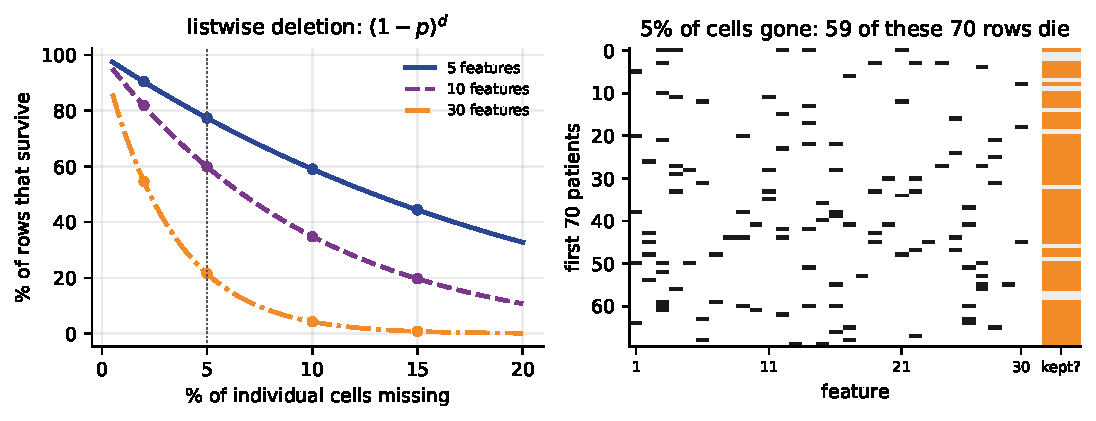
\includegraphics[width=0.92\textwidth]{listwise.pdf}
  \end{center}
  \begin{center}\small
    Left: $(1-p)^d$, measured against the formula. At $p = 5\%$ five columns
    keep $77\%$ of rows and thirty columns keep $21\%$. Right: the actual
    mask. Black cells are missing; the orange strip is the verdict.
    \textbf{Fifty-nine of these seventy patients die of one missing number.}
  \end{center}
\end{frame}

\begin{frame}[fragile,shrink=4]{Was deleting them at least \emph{safe}?}
\begin{outblk}
accuracy on the 114 survivors             0.9735  +/- 0.0216
accuracy imputing instead, all 569 rows   0.9719  +/- 0.0129
baseline with no missingness at all       0.9807  +/- 0.0065
\end{outblk}
\onslide<2->
\begin{columns}[T]
  \begin{column}{0.5\textwidth}
    \begin{block}{Be honest about this}
      \small On \emph{this} easy dataset deletion did not lose accuracy. It
      lost \textbf{455 patients} and widened the spread of the estimate by
      $1.7\times$.
    \end{block}
  \end{column}
  \begin{column}{0.46\textwidth}
    \begin{alertblock}{It is not always this kind}
      \small On \texttt{load\_diabetes} at $30\%$ missing, listwise deletion
      leaves \textbf{9 training rows} for $10$ features and the fitted model
      scores $R^2 = -4.70$.
    \end{alertblock}
  \end{column}
\end{columns}
\onslide<3->
\begin{center}\small
  \textbf{Deletion is a decision to throw away evidence.} Sometimes it is the
  right one. It is never the free one.
\end{center}
\end{frame}

% =====================================================================
\section[Missing]{Handling missing data}
\label{sec:missing}

\begin{frame}[shrink=6]{Three questions to ask about a hole}
  \begin{enumerate}
    \item<1-> \textbf{Why is it missing?} A sensor failed, a question was
      refused, a test was never ordered --- three different problems with
      three different fixes.
    \item<2-> \textbf{Is the reason related to the value itself?} This is the
      MCAR / MAR / MNAR question, and it decides whether \emph{any} imputer
      can save you.
    \item<3-> \textbf{Is the \emph{fact} of the hole informative?} If a test
      is ordered only for patients who already look ill, then
      \texttt{isnull()} is a feature.
  \end{enumerate}
  \vspace{0.6em}
  \onslide<4->{
  \begin{alertblock}{The mistake this section exists to prevent}
    \centering\small
    Reaching for \texttt{fillna(df.mean())} without asking any of the three.
  \end{alertblock}}
\end{frame}

\begin{frame}[shrink=8]{By hand: eight marks, two missing}
  \[
    55,\ 62,\ \boxed{?},\ 71,\ 58,\ \boxed{?},\ 90,\ 64
  \]
  Sort the six we have: $55,\ 58,\ 62,\ 64,\ 71,\ 90$.
  \begin{center}\small
  \begin{tabular}{@{}llr@{}}
    \toprule
    mean   & $(55+62+71+58+90+64)/6 = 400/6$ & $66.6667$\\
    median & $(62+64)/2$                     & $63.0000$\\
    sd ($n-1$) & $\sqrt{\frac{1}{5}\sum (x_i-\bar x)^2}$ & $12.6754$\\
    \bottomrule
  \end{tabular}
  \end{center}
  \vspace{0.3em}
  \begin{exampleblock}{Mean, median or mode?}
    \small \textbf{Mean} for a symmetric numeric column. \textbf{Median} when
    it is skewed --- here $90$ drags the mean $3.7$ marks above the median.
    \textbf{Mode} for a categorical column, where a mean is meaningless.
  \end{exampleblock}
\end{frame}

\begin{frame}[shrink=6]{By hand: what mean imputation does to the spread}
  Fill both holes with $\bar x$. The mean cannot move --- you added two copies
  of it. The \emph{sum of squared deviations} cannot move either, because the
  two new deviations are zero. But you now divide it among more values:
  \[
    \sigma^2_{\text{after}}
    = \frac{\sum_{i=1}^{m}(x_i - \bar x)^2}{n}
    = \frac{m}{n}\,\sigma^2_{\text{before}}
    \qquad\Longrightarrow\qquad
    \frac{\sigma_{\text{after}}}{\sigma_{\text{before}}} = \sqrt{\frac{m}{n}}
    = \sqrt{1-p}.
  \]
  \begin{center}\small
    Here $m = 6$ observed of $n = 8$, so the population variance is multiplied
    by $6/8 = 0.75$ and the sample variance by $(m-1)/(n-1) = 5/7 = 0.7143$.
  \end{center}
  \begin{alertblock}{This is not an approximation}
    \small It is exact, and it is the reason mean imputation is the worst
    defensible thing you can do. \textbf{You have invented confidence you do
    not have.}
  \end{alertblock}
\end{frame}

\begin{frame}[fragile]{The same thing in code}
\begin{lstlisting}
marks = np.array([55, 62, np.nan, 71, 58, np.nan, 90, 64])
obs = marks[~np.isnan(marks)]
for name, fill in (("mean", obs.mean()), ("median", np.median(obs))):
    f = np.where(np.isnan(marks), fill, marks)
    print(name, f.mean(), f.std(ddof=1))
\end{lstlisting}
\begin{outblk}
mean of observed         66.6667
median of observed       63.0000
sd of observed (ddof=1)  12.6754
mean   imputed:  mean 66.6667   sd 10.7127   sd is now 84.5% of the truth
median imputed:  mean 65.7500   sd 10.8463   sd is now 85.6% of the truth
\end{outblk}
\begin{center}\small
  $10.7127/12.6754 = 0.8452$, and $\sqrt{5/7} = 0.8452$. The formula and the
  library agree to four decimal places, because they are the same arithmetic.
\end{center}
\end{frame}

\begin{frame}[fragile,shrink=10]{Predict first \#2}
Take a real column --- body mass index for the $442$ diabetes patients,
sd $= 4.42\ \mathrm{kg/m^2}$. Hide \textbf{40\%} of it at random and fill every
hole with the mean of what is left.

\begin{center}
  \textbf{What is the standard deviation now? And what happens to its
  correlation with the target?}
\end{center}
\vspace{0.3em}
\onslide<2->
\begin{outblk}
  p=0.1   measured sd ratio 0.9486   sqrt(1-p) = 0.9487
  p=0.3   measured sd ratio 0.8363   sqrt(1-p) = 0.8367
  p=0.5   measured sd ratio 0.7059   sqrt(1-p) = 0.7071
  p=0.7   measured sd ratio 0.5447   sqrt(1-p) = 0.5477
  complete data       corr(BMI, y) = 0.5865
  40% mean-imputed    corr(BMI, y) = 0.4538  (77% of it survives)
\end{outblk}
\onslide<3->
\begin{alertblock}{The variance shrinks by $1-p$, and a quarter of the signal goes}
  \footnotesize Four values of $p$, $2000$ repetitions each, never more than
  $0.0031$ from $\sqrt{1-p}$. \textbf{Every correlation, every regression
  coefficient and every $p$-value computed afterwards is attenuated}, and
  nothing in the output warns you.
\end{alertblock}
\end{frame}

\begin{frame}[shrink=8]{Drawn: a spike where a distribution used to be}
  \begin{center}
    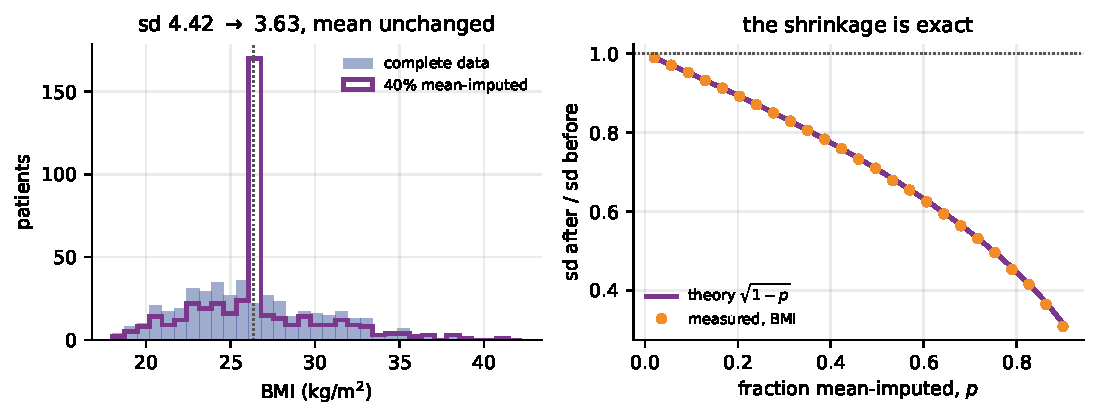
\includegraphics[width=0.90\textwidth]{shrink.pdf}
  \end{center}
  \begin{center}\small
    Left: the same column before and after. Mean imputation does not blur the
    distribution --- it \textbf{piles every hidden patient onto a single
    value}, $4.4181 \rightarrow 3.6309$. Right: the average of $400$ draws
    per point against $\sqrt{1-p}$, largest disagreement $0.0080$ over the
    whole range.
  \end{center}
\end{frame}

\begin{frame}[shrink=6]{MCAR, MAR, MNAR: the taxonomy that matters}
  Write $R$ for the indicator ``this value is missing'', $X_{\text{obs}}$ for
  what you can see and $X_{\text{mis}}$ for what you cannot.
  \begin{center}\small
  \begin{tabular}{@{}llp{5.2cm}@{}}
    \toprule
    & \textbf{Depends on} & \textbf{Example}\\
    \midrule
    \textbf{MCAR} & nothing:
      $P(R) $ constant & a tube was dropped in the lab\\[3pt]
    \textbf{MAR}  & $X_{\text{obs}}$ only &
      BMI recorded only for the high-blood-pressure patients\\[3pt]
    \textbf{MNAR} & $X_{\text{mis}}$ itself &
      the heaviest patients decline to be weighed\\
    \bottomrule
  \end{tabular}
  \end{center}
  \vspace{0.3em}
  \begin{exampleblock}{Why you should care}
    \small Under \textbf{MCAR} the complete cases are a fair sample --- you
    lose power, not correctness. Under \textbf{MAR} a good imputer that uses
    the other columns can recover the truth. Under \textbf{MNAR} \emph{nothing
    in the data} can, because the information you need was never recorded.
  \end{exampleblock}
\end{frame}

\begin{frame}[fragile,shrink=4]{The three mechanisms, measured}
Same column, same $40$--$48\%$ missing, three different reasons:
\begin{lstlisting}
rng  = np.random.default_rng(0)        # the one seed for this lecture
mcar = rng.random(n) < 0.40            # a coin
mar  = bp < np.median(bp)              # depends on BP, which we can see
mnar = bmi > np.quantile(bmi, 0.60)    # depends on BMI itself
\end{lstlisting}
\begin{outblk}
complete-data mean BMI  26.3758 kg/m2   (n = 442)
  MCAR  35.3% missing   complete-case mean 26.4913   bias +0.1155
  MAR   48.0% missing   complete-case mean 27.7230   bias +1.3473
  MNAR  40.0% missing   complete-case mean 23.4253   bias -2.9505
\end{outblk}
\onslide<2->
\begin{center}\small
  Throwing away the incomplete rows is \emph{almost} free under MCAR
  ($+0.12$, and it would change sign with another draw), wrong by $+1.35$
  under MAR, and wrong by $-2.95$ under MNAR --- \textbf{two thirds of a
  standard deviation}, from a decision you never made.
\end{center}
\end{frame}

\begin{frame}[shrink=8]{Drawn: the same histogram, three ways of losing it}
  \begin{center}
    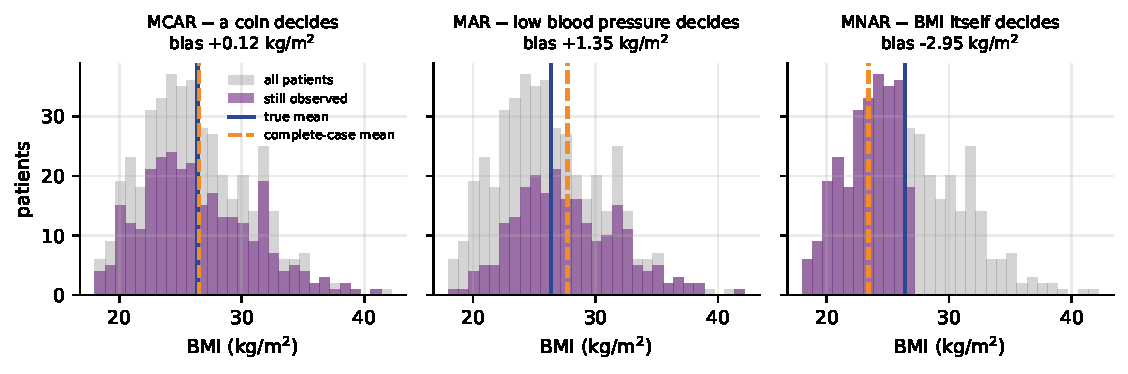
\includegraphics[width=0.94\textwidth]{mechanisms.pdf}
  \end{center}
  \begin{center}\small
    Grey is everyone; purple is who is left. Under MCAR the purple bars are a
    shrunken copy of the grey. Under MNAR the right-hand tail is
    \textbf{simply gone}, and no amount of cleverness puts it back.
  \end{center}
\end{frame}

\begin{frame}[fragile]{Can a better imputer repair it?}
\texttt{IterativeImputer} (MICE) predicts each column from all the others,
round-robin, until it settles.
\begin{outblk}
  MCAR mean     imputed mean 26.4913   bias +0.1155
  MCAR MICE     imputed mean 26.4763   bias +0.1005
  MAR  mean     imputed mean 27.7230   bias +1.3473
  MAR  MICE     imputed mean 26.2170   bias -0.1588
  MNAR mean     imputed mean 23.4253   bias -2.9505
  MNAR MICE     imputed mean 23.7924   bias -2.5834
\end{outblk}
\onslide<2->
\begin{alertblock}{Read the middle pair, then the last pair}
  \footnotesize Under MAR, MICE cuts the bias from $+1.35$ to $-0.16$ --- an
  \textbf{$8.5\times$ improvement}, because blood pressure was recorded and
  BMI can be predicted from it. Under MNAR it moves $-2.95$ to $-2.58$ and
  stops. \textbf{The taxonomy is not academic: it tells you whether to bother.}
\end{alertblock}
\end{frame}

\begin{frame}[fragile,shrink=4]{And what it does to a coefficient you would report}
Regress the target on all ten features and read off the BMI coefficient.
\begin{outblk}
  true BMI coefficient             5.603
  MNAR + mean imputation          -0.413
  MNAR + MICE                      2.299
\end{outblk}
\onslide<2->
\begin{alertblock}{The sign flipped}
  \footnotesize Mean-imputing an MNAR column does not merely weaken the
  relationship. It replaces the entire upper $40\%$ of the distribution with
  one constant, and the fitted slope through what remains points the
  \emph{other way}. \textbf{You would have written ``BMI is unrelated to
  disease progression'' in a report.}
\end{alertblock}
\onslide<3->
\begin{center}\small
  Prediction is more forgiving than inference --- but only because nobody
  reads a predictor's coefficients.
\end{center}
\end{frame}

\begin{frame}[fragile,shrink=6]{So which imputer should you use?}
\texttt{load\_diabetes}, holes punched in the \emph{training} matrix only,
clean test set, 20 random splits:
\begin{outblk}
                          10% missing        30% missing
  oracle, no missingness  0.4762            0.4762
  drop incomplete rows    0.4264           -4.6952  (+/- 7.88)
  mean                    0.4721            0.4351
  median                  0.4727            0.4364
  constant 0              0.4723            0.4365
  KNN, k=5                0.4743            0.4591
  iterative (MICE)        0.4751            0.2639  (+/- 0.50)
\end{outblk}
\onslide<2->
\begin{alertblock}{Deletion costs 0.05; the choice of imputer costs 0.003}
  \footnotesize At $10\%$ every imputer lands within $0.003$ of every other and
  within $0.004$ of the oracle. \textbf{Do not agonise over the imputer. Do not
  drop the rows.} At $30\%$, KNN pulls ahead --- and MICE became unstable on
  two of twenty splits, which is why its error bar is a factor of ten larger.
\end{alertblock}
\end{frame}

\begin{frame}[shrink=8]{Drawn: the same table}
  \begin{center}
    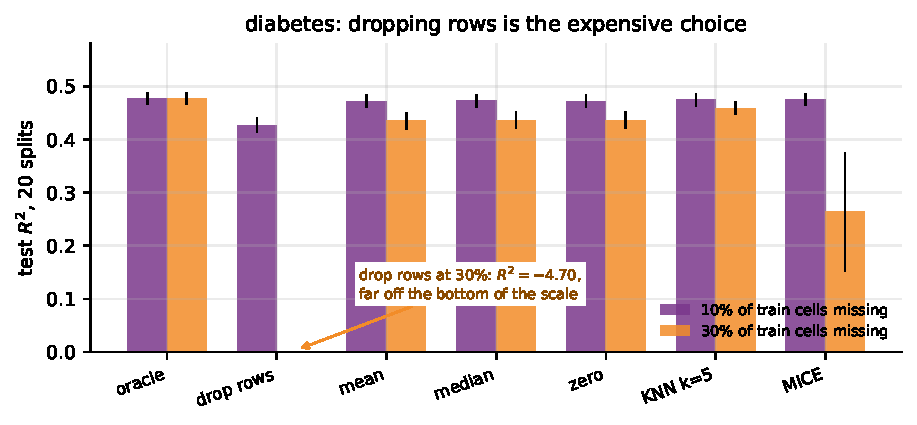
\includegraphics[width=0.78\textwidth]{imputescores.pdf}
  \end{center}
  \begin{center}\small
    Purple $10\%$, orange $30\%$; error bars are standard errors over $20$
    splits. Six of the seven bars are the same height. The one that is not is
    the one everybody's first instinct reaches for.
  \end{center}
\end{frame}

\begin{frame}[fragile,shrink=4]{Missingness is itself data}
A weak feature, missing $80\%$ of the time for one class and $20\%$ for the
other --- a test ordered only when the clinician already suspects something.
\begin{lstlisting}
SimpleImputer(strategy="mean", add_indicator=True)
\end{lstlisting}
\begin{outblk}
  mean imputation only          0.6294
  mean imputation + indicator   0.7969
  difference                   +0.1675
\end{outblk}
\onslide<2->
\begin{columns}[T]
  \begin{column}{0.5\textwidth}
    \begin{exampleblock}{Sixteen points of accuracy}
      \small from a column of \texttt{True}/\texttt{False} that you get for
      free with one keyword argument.
    \end{exampleblock}
  \end{column}
  \begin{column}{0.46\textwidth}
    \begin{alertblock}{And a warning}
      \small If the reason for the hole will not exist at prediction time,
      that indicator is \textbf{leakage}, not a feature.
    \end{alertblock}
  \end{column}
\end{columns}
\end{frame}

% =====================================================================
\section[Outliers]{Handling outliers}
\label{sec:outliers}

\begin{frame}[shrink=6]{Three kinds of outlier, one word}
  \begin{columns}[T]
    \begin{column}{0.31\textwidth}
      \begin{block}{An error}
        Age $= 200$. A stuck sensor. A pressure in the wrong units.\\[0.3em]
        \textbf{Fix or remove it.}
      \end{block}
    \end{column}
    \begin{column}{0.31\textwidth}
      \begin{block}{A rare truth}
        A genuine very large tumour. \\[0.3em]
        \textbf{Keep it. Use a robust method.}
      \end{block}
    \end{column}
    \begin{column}{0.31\textwidth}
      \begin{exampleblock}{The point}
        Fraud. A failing machine. A new phenomenon.\\[0.3em]
        \textbf{It is the signal.}
      \end{exampleblock}
    \end{column}
  \end{columns}
  \vspace{0.5em}
  \begin{alertblock}{No statistical rule can tell these three apart}
    A rule tells you a point is \emph{unusual}. Only domain knowledge tells you
    what to do about it. \textbf{Detection is statistics; disposal is a
    judgement you must be able to defend.}
  \end{alertblock}
  \vspace{0.2em}
  \begin{center}\small
    Iglewicz and Hoaglin's three words: \emph{labelling}, \emph{accommodation},
    \emph{identification}. Today is mostly labelling.
  \end{center}
\end{frame}

\begin{frame}[shrink=8]{Three rules you will meet}
  \begin{center}\small
  \begin{tabular}{@{}lllp{2.9cm}@{}}
    \toprule
    & \textbf{Statistic} & \textbf{Flag when} & \textbf{Breakdown point}\\
    \midrule
    $z$-score & $z_i = \dfrac{x_i-\bar x}{s}$ & $|z_i| > 3$ &
      $0\%$: one point moves both $\bar x$ and $s$\\[8pt]
    Tukey / IQR & $\mathrm{IQR}=Q_3-Q_1$ &
      outside $Q_{1,3} \mp 1.5\,\mathrm{IQR}$ & $25\%$\\[8pt]
    modified $z$ & $M_i = \dfrac{0.6745\,(x_i-\tilde x)}{\mathrm{MAD}}$ &
      $|M_i| > 3.5$ & $50\%$: median and MAD\\
    \bottomrule
  \end{tabular}
  \end{center}
  \vspace{0.4em}
  \begin{block}{Where the two magic constants come from}
    \small $\mathrm{MAD} = \operatorname{median}|x_i - \tilde x|$. For Normal
    data $\mathrm{MAD} \approx 0.6745\,\sigma$, so dividing by $0.6745$ puts
    $M$ back on the $z$ scale. The $1.5$ in Tukey's fence flags
    $0.70\%$ of Normal data; $|z|>3$ flags $0.27\%$.
  \end{block}
\end{frame}

\begin{frame}[shrink=8]{By hand: thirty-five readings from one sensor}
  Thirty genuine readings scattered around $10.0$, then the sensor sticks and
  reports $100.0$ five times.
  \begin{center}\small
  \begin{tabular}{@{}lrlr@{}}
    \toprule
    mean $\bar x$ & $22.503$ & median $\tilde x$ & $9.950$\\
    sd $s$        & $32.109$ & MAD               & $0.540$\\
    $Q_1$         & $9.245$  & $Q_3$             & $10.330$\\
    \bottomrule
  \end{tabular}
  \end{center}
  \vspace{0.2em}
  Now score one stuck reading, $x = 100$, with each rule:
  \[
    z = \frac{100 - 22.503}{32.109} = 2.4135,
    \qquad
    M = \frac{0.6745\,(100 - 9.950)}{0.540} = 112.48 .
  \]
  \begin{alertblock}{$2.41$ against a threshold of $3$}
    \small The five stuck readings dragged $\bar x$ from $9.59$ up to $22.50$
    and inflated $s$ from $0.84$ to $32.11$. \textbf{They are being measured
    against a ruler they themselves bent.}
  \end{alertblock}
\end{frame}

\begin{frame}[fragile,shrink=8]{Predict first \#3}
Thirty good readings near $10$. Five readings of exactly $100$ --- as wrong as
a reading can be, and you can see them from across the room.

\begin{center}
  \textbf{How many of the five does the $|z| > 3$ rule catch? What about the
  IQR fence and the modified $z$?}
\end{center}
\vspace{0.3em}
\onslide<2->
\begin{outblk}
rule                     flags   of which stuck   of which genuine
  |z| > 3                  0          0               0
  outside 1.5*IQR fence    6          5               1
  |modified z| > 3.5       5          5               0
sd WITHOUT the five stuck readings  0.837
z of a stuck reading would then be  108.1
\end{outblk}
\onslide<3->
\begin{alertblock}{Zero. The most-taught rule in the subject finds none of them}
  \footnotesize And it is not close: $2.41$ against $3$. Remove the outliers
  first and the very same reading scores $z = 108$. \textbf{This is
  \emph{masking}: an outlier inflates the standard deviation it is being
  divided by, and hides inside its own damage.}
\end{alertblock}
\end{frame}

\begin{frame}[fragile,shrink=4]{The same thing in code}
\begin{lstlisting}
z   = (v - v.mean()) / v.std(ddof=1)
q1, q3 = np.percentile(v, [25, 75]);  iqr = q3 - q1
mad = np.median(np.abs(v - np.median(v)))
mz  = 0.6745 * (v - np.median(v)) / mad
\end{lstlisting}
\begin{outblk}
  mean 22.503   sd 32.109   median 9.950   MAD 0.540
  Q1 9.245  Q3 10.330  IQR 1.085  upper fence Q3+1.5*IQR 11.957
  a stuck reading:  z = 2.4135  (needs > 3)   modified z = 112.48  (needs > 3.5)
\end{outblk}
\onslide<2->
\begin{center}\small
  Four lines each. The whole difference is that the middle rule uses
  \textbf{quartiles} and the third uses \textbf{a median and a median} --- and
  a median does not care how far away the far-away points are.
\end{center}
\end{frame}

\begin{frame}[shrink=8]{Drawn: masking, and why it gets worse}
  \begin{center}
    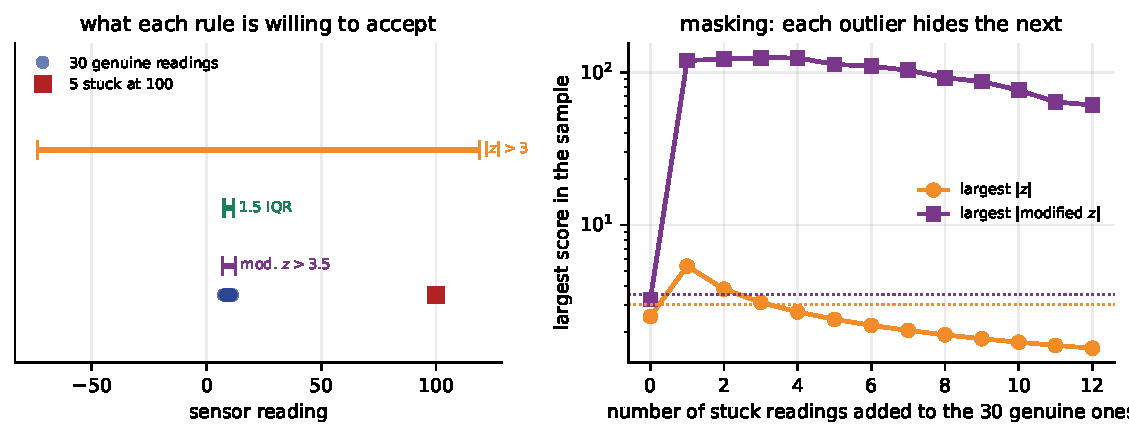
\includegraphics[width=0.92\textwidth]{masking.pdf}
  \end{center}
  \begin{center}\small
    Left: what each rule is willing to accept. The $z$ interval reaches from
    $-74$ to $+119$; the other two are slivers around $10$. Right: add stuck
    readings one at a time. \textbf{One outlier is caught at $z = 5.38$, two at
    $3.81$, three at $3.11$, and from the fourth onwards none ever again.}
    The modified $z$ stays above $60$ throughout.
  \end{center}
\end{frame}

\begin{frame}[fragile,shrink=4]{By hand: the rule has a ceiling}
For a sample of $n$ values with sample standard deviation $s$ (the $n-1$ one),
no observation can have
\[
  |z| > \frac{n-1}{\sqrt{n}} .
\]
\begin{outblk}
 n   largest possible |z|   can the rule |z| > 3 ever fire?
  3        1.1547              NO -- not ever
  5        1.7889              NO -- not ever
 10        2.8460              NO -- not ever
 11        3.0151              yes
 50        6.9296              yes
\end{outblk}
\onslide<2->
\begin{alertblock}{Below $n = 11$ the rule is not strict --- it is inert}
  \footnotesize Whatever the data, whatever the contamination. If you have ten
  measurements and you apply $|z|>3$, you have written a line of code that can
  only ever return ``no outliers''. NIST states the bound in exactly these
  words, and the fix in the next line: use the modified $z$.
\end{alertblock}
\end{frame}

\begin{frame}[shrink=8]{Drawn: the ceiling}
  \begin{center}
    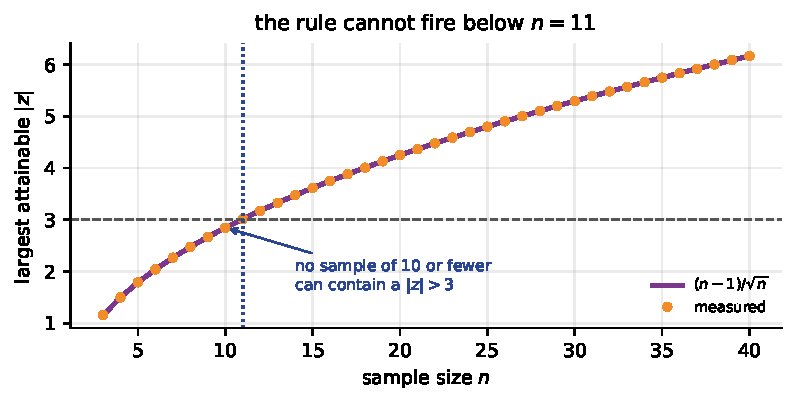
\includegraphics[width=0.62\textwidth]{maxz.pdf}
  \end{center}
  \begin{center}\small
    Theory and measurement agree to $9\times10^{-16}$. The curve crosses $3$
    between $n = 10$ ($2.846$) and $n = 11$ ($3.015$). \textbf{The threshold
    that everybody memorises has a domain of validity that nobody mentions.}
  \end{center}
\end{frame}

\begin{frame}[fragile,shrink=6]{The opposite failure: a skewed column}
The most skewed column of \texttt{load\_breast\_cancer} --- \texttt{'area
error'}, skewness $5.43$, no contamination at all.
\begin{outblk}
  rule                  flags     % of rows
  |z| > 3                  6         1.1%
  1.5*IQR fences          65        11.4%
  |modified z| > 3.5      81        14.2%
  under a perfect Normal these rules flag 0.27%, 0.70% and 0.35% of rows
\end{outblk}
\onslide<2->
\begin{outblk}
  now Yeo-Johnson the column first (skewness 5.433 -> 0.069) and repeat
  |z| > 3                  0         0.0%
  1.5*IQR fences           1         0.2%
  |modified z| > 3.5       0         0.0%
\end{outblk}
\onslide<3->
\begin{alertblock}{Eighty-one ``outliers'' that were never outliers}
  \footnotesize Every one of these rules assumes symmetry. On a long right
  tail they flag the tail. \textbf{Transform first, then look for outliers} ---
  and that is the whole argument for the next section.
\end{alertblock}
\end{frame}

\begin{frame}[shrink=8]{Drawn: skew looks exactly like contamination}
  \begin{center}
    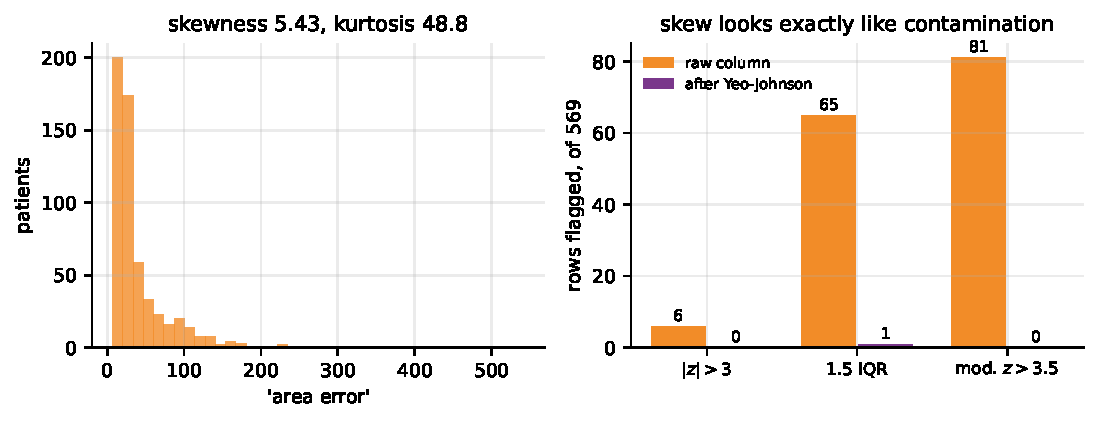
\includegraphics[width=0.90\textwidth]{rules.pdf}
  \end{center}
  \begin{center}\small
    Left: the raw column, kurtosis $48.8$. Right: how many rows each rule
    condemns before and after a single power transform.
    $6 \rightarrow 0$, $65 \rightarrow 1$, $81 \rightarrow 0$ --- and not one
    data value was deleted.
  \end{center}
\end{frame}

\begin{frame}[shrink=6]{Numerical methods, 1: binning and smoothing}
  Nine sorted prices, three equal-depth bins. This is Han, Kamber and Pei's
  standard treatment of \emph{noisy} data, and it is a favourite exam question.
  \begin{center}\small
  \begin{tabular}{@{}llrrl@{}}
    \toprule
    Bin & Values & mean & median & boundaries\\
    \midrule
    1 & $4,\ 8,\ 15$   & $9$  & $8$  & $4$ and $15$\\
    2 & $21,\ 21,\ 24$ & $22$ & $21$ & $21$ and $24$\\
    3 & $25,\ 28,\ 34$ & $29$ & $28$ & $25$ and $34$\\
    \bottomrule
  \end{tabular}
  \end{center}
  \vspace{0.2em}
  \begin{center}\small
  \begin{tabular}{@{}ll@{}}
    \toprule
    by bin \textbf{means}      & $9,\ 9,\ 9,\ 22,\ 22,\ 22,\ 29,\ 29,\ 29$\\
    by bin \textbf{medians}    & $8,\ 8,\ 8,\ 21,\ 21,\ 21,\ 28,\ 28,\ 28$\\
    by bin \textbf{boundaries} & $4,\ 4,\ 15,\ 21,\ 21,\ 24,\ 25,\ 25,\ 34$\\
    \bottomrule
  \end{tabular}
  \end{center}
  \vspace{0.2em}
  \begin{block}{Read the third row}
    \small Each value is replaced by whichever \emph{end} of its bin is closer:
    $8$ is nearer $4$ than $15$, so it becomes $4$; $15$ stays $15$.
  \end{block}
\end{frame}

\begin{frame}[fragile,shrink=6]{Numerical methods, 2: five things to do to an outlier}
Back to the thirty-five sensor readings. The truth is mean $9.586$,
sd $0.837$.
\begin{outblk}
  leave them alone         mean  22.503   sd  32.109   n 35
  winsorise at 5 and 95    mean  22.523   sd  32.100   n 35
  winsorise at 15 and 85   mean   9.903   sd   0.839   n 35
  cap at the IQR fence     mean   9.925   sd   1.143   n 35
  drop by modified z       mean   9.586   sd   0.837   n 30
  the 30 genuine readings  mean   9.586   sd   0.837   n 30
\end{outblk}
\onslide<2->
\begin{alertblock}{Look at the second row before anything else}
  \footnotesize Winsorising at the $5$th and $95$th percentiles did
  \textbf{nothing}, because $5/35 = 14\%$ of the data is contaminated and you
  told it to clip $10\%$. \textbf{A fixed percentile is a guess about how much
  dirt there is.} The IQR fence and the modified $z$ work it out from the data.
\end{alertblock}
\end{frame}

\begin{frame}[fragile,shrink=4]{And the scaler you choose is an outlier decision}
\begin{lstlisting}
StandardScaler().fit_transform(sensor.reshape(-1, 1))   # (x - mean) / sd
RobustScaler().fit_transform(sensor.reshape(-1, 1))     # (x - median) / IQR
\end{lstlisting}
\begin{outblk}
  StandardScaler  30 genuine readings span -0.4747 to -0.3527  (width 0.1220)
  RobustScaler    30 genuine readings span -2.2765 to  1.2811  (width 3.5576)
\end{outblk}
\onslide<2->
\begin{center}\small
  \textbf{The same thirty readings, squashed into $0.12$ of a unit or spread
  over $3.56$.} \texttt{StandardScaler} spent its whole dynamic range
  accommodating five wrong numbers, and every distance-based model downstream
  now thinks those thirty patients are identical.
\end{center}
\end{frame}

% =====================================================================
\section[Transform]{Data transformation}
\label{sec:transform}

\begin{frame}[shrink=6]{Why transform a variable at all}
  \begin{columns}[T]
    \begin{column}{0.48\textwidth}
      \begin{block}{Four honest reasons}
        \begin{enumerate}\small
          \item Symmetry: a mean and an sd stop lying.
          \item Linearity: a curved relationship straightens.
          \item Equal spread: residual variance stops growing with the fit.
          \item Outlier rules start working (previous section).
        \end{enumerate}
      \end{block}
    \end{column}
    \begin{column}{0.48\textwidth}
      \begin{exampleblock}{The ladder of powers}
        \small
        $\dots,\ -1/x,\ -1/\sqrt x,\ \log x,\ \sqrt x,\ x,\ x^2,\ \dots$\\[0.3em]
        Move \textbf{down} to pull in a right tail, \textbf{up} for a left
        one. $\log$ sits in the middle and is the one you will use most.
      \end{exampleblock}
    \end{column}
  \end{columns}
  \vspace{0.3em}
  \begin{alertblock}{Two things a transform is not}
    \small It is not scaling (that is L6, and it does not change shape). And it
    is not free: after $\log$, a coefficient is a statement about
    \emph{percentage} change, and you must say so.
  \end{alertblock}
\end{frame}

\begin{frame}[fragile,shrink=6]{Four transformations, one real column}
\texttt{'area error'}: $569$ values, minimum $6.80$, maximum $542.2$.
\begin{outblk}
  transformation        skewness    kurtosis
  none                    5.4328    48.7672
  sqrt(x)                 2.1363     7.8193
  log(x)                  0.7955     0.3622
  1/sqrt(x)               0.0447    -0.3685
  Box-Cox, lam=-0.436     0.0584    -0.4094
  Yeo-Johnson             0.0691    -0.4561
\end{outblk}
\onslide<2->
\begin{center}\small
  Skewness $5.43 \rightarrow 0.06$, kurtosis $48.8 \rightarrow -0.41$. The
  square root was not enough; the log almost was; the reciprocal square root
  went slightly past.
\end{center}
\onslide<3->
\begin{alertblock}{The ladder is discrete, and the right rung is between two of them}
  \footnotesize That is precisely the gap Box--Cox fills.
\end{alertblock}
\end{frame}

\begin{frame}[shrink=8]{Drawn: the same 569 numbers, four ways}
  \begin{center}
    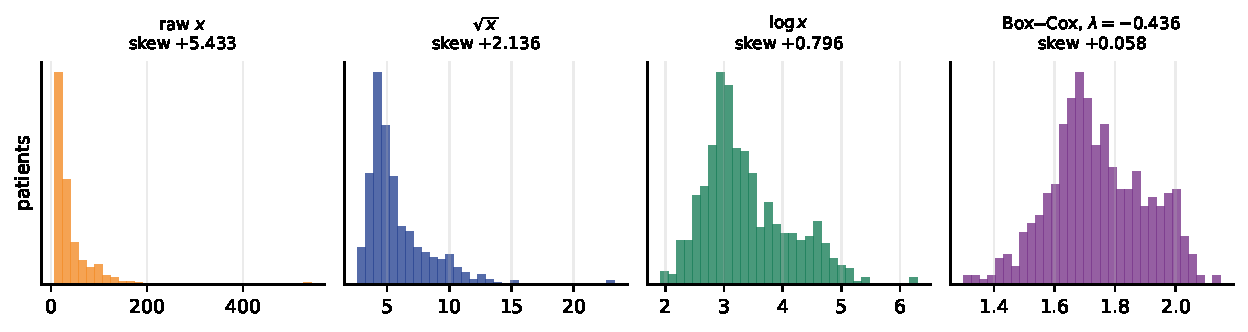
\includegraphics[width=0.98\textwidth]{transforms.pdf}
  \end{center}
  \begin{center}\small
    Nothing has been deleted and no value has changed its rank. All that
    changed is the ruler the values are printed on --- and the fourth panel is
    a variable you can put a mean and a standard deviation on.
  \end{center}
\end{frame}

\begin{frame}[shrink=6]{Box--Cox and Yeo--Johnson}
  \[
    x^{(\lambda)} =
    \begin{cases}
      \dfrac{x^{\lambda}-1}{\lambda}, & \lambda \neq 0\\[8pt]
      \log x, & \lambda = 0
    \end{cases}
    \qquad\qquad x > 0 \text{ required}
  \]
  \begin{columns}[T]
    \begin{column}{0.48\textwidth}
      \begin{block}{Why the $-1$ and the $/\lambda$}
        \small So that the family is \emph{continuous} at $\lambda = 0$:
        $(x^\lambda-1)/\lambda \to \log x$. Without them, $\lambda \to 0$ would
        give the constant $1$.
      \end{block}
    \end{column}
    \begin{column}{0.48\textwidth}
      \begin{exampleblock}{Yeo--Johnson}
        \small The same idea rewritten so that it works for $x \le 0$: it
        applies the Box--Cox form to $x+1$ on the positive side and a mirrored
        version to $-x+1$ on the negative side.
      \end{exampleblock}
    \end{column}
  \end{columns}
  \vspace{0.3em}
  \begin{center}\small
    $\lambda$ is chosen by \textbf{maximum likelihood} under a Normal model,
    not by minimising skewness --- which is why the two answers differ slightly.
  \end{center}
\end{frame}

\begin{frame}[fragile,shrink=6]{$\lambda$ chooses a rung of the ladder}
\begin{outblk}
  lambda -1.00   1/x  (reciprocal)  skewness  -0.8635
  lambda -0.50   1/sqrt(x)          skewness  -0.0447
  lambda +0.00   log(x)             skewness  +0.7955
  lambda +0.50   sqrt(x)            skewness  +2.1363
  lambda +1.00   x  (no change)     skewness  +5.4328
  maximum-likelihood lambda from scipy   -0.4357
  skewness there                         +0.0584
\end{outblk}
\onslide<2->
\begin{outblk}
a column that goes negative cannot use Box-Cox
  diabetes 'bp': min -0.1124  max 0.1320  skewness +0.2897
  stats.boxcox(bp) -> ValueError: Data must be positive.
  Yeo-Johnson handles it: skewness +0.2897 -> +0.0226
\end{outblk}
\onslide<3->
\begin{center}\small
  \textbf{Every rung you know is a value of $\lambda$}, and $\lambda$ is
  allowed to be $-0.4357$.
\end{center}
\end{frame}

\begin{frame}[shrink=8]{Drawn: what scipy is actually maximising}
  \begin{center}
    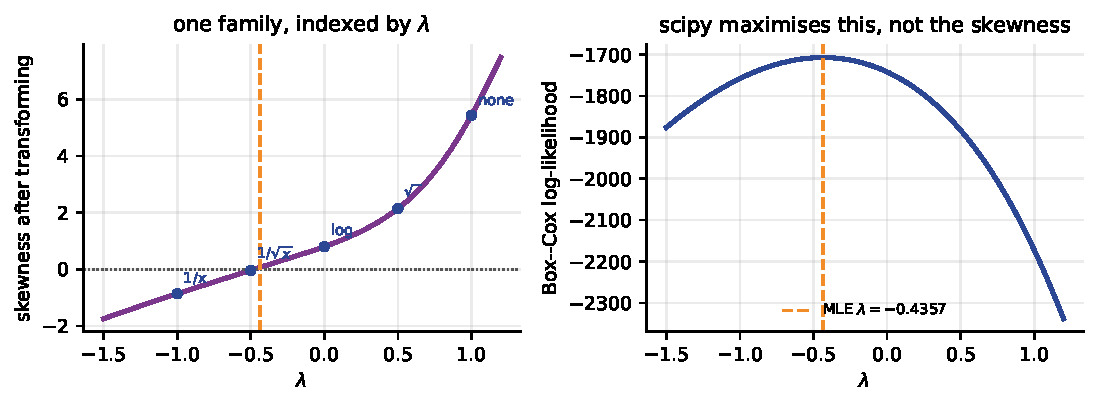
\includegraphics[width=0.90\textwidth]{boxcox.pdf}
  \end{center}
  \begin{center}\small
    Left: skewness against $\lambda$, with the five named rungs marked. Right:
    the Box--Cox log-likelihood, whose peak is at $\lambda = -0.4357$. The
    $\lambda$ that would zero the skewness exactly is $-0.4688$ --- close, but
    they are answers to different questions.
  \end{center}
\end{frame}

\begin{frame}[fragile,shrink=4]{Does it help the model? It depends which model}
20 random splits of \texttt{load\_breast\_cancer}:
\begin{outblk}
  GaussianNB           scale only 0.9304   Yeo-Johnson first 0.9462   +0.0157  (16/20)
  LogisticRegression   scale only 0.9762   Yeo-Johnson first 0.9766   +0.0003  (5/20)
\end{outblk}
\onslide<2->
\begin{columns}[T]
  \begin{column}{0.5\textwidth}
    \begin{exampleblock}{Naive Bayes gains 1.6 points}
      \small It \emph{assumes} each feature is Normal within a class. Making
      that assumption true is worth real accuracy, on 16 of the 20 splits.
    \end{exampleblock}
  \end{column}
  \begin{column}{0.46\textwidth}
    \begin{alertblock}{Logistic regression gains nothing}
      \small It makes no distributional assumption about $X$ at all.
      \textbf{$+0.0003$ is noise, and it won 5 splits of 20.}
    \end{alertblock}
  \end{column}
\end{columns}
\onslide<3->
\begin{center}\small
  \textbf{Transform because the model assumes it, or because you need to read
  the variable} --- not as a ritual.
\end{center}
\end{frame}

% =====================================================================
\section[Order]{The order of operations}
\label{sec:leak}

\begin{frame}[shrink=6]{The single rule that governs all of it}
  \begin{exampleblock}{}
    \centering \large
    Every number used to clean the data must be computed from the
    \textbf{training rows only}.
  \end{exampleblock}
  \vspace{0.4em}
  \begin{center}\small
  \begin{tabular}{@{}ll@{}}
    \toprule
    \textbf{Step} & \textbf{The number it learns}\\
    \midrule
    imputation & the column mean, median, mode, or a fitted model\\
    outlier removal & a threshold, or \emph{which rows to keep}\\
    transformation & $\lambda$\\
    scaling & the mean and the standard deviation\\
    \bottomrule
  \end{tabular}
  \end{center}
  \vspace{0.3em}
  \begin{alertblock}{Break it and your test score is a measurement of nothing}
    \small The score you report is no longer an estimate of performance on
    unseen data, because the data was not unseen. \textbf{How much you
    overstate by depends entirely on which step you got wrong} --- and the
    range is enormous.
  \end{alertblock}
\end{frame}

\begin{frame}[fragile,shrink=6]{Predict first \#4}
The most human thing in data science: fit a model, look at the rows it gets
badly wrong, decide they are outliers, delete them, and start again.

Concretely: fit on all $442$ diabetes patients, delete the $10\%$ with the
largest residual, \emph{then} split into train and test and report $R^2$.

\begin{center}
  \textbf{By how much does that overstate the honest number?}
\end{center}
\vspace{0.3em}
\onslide<2->
\begin{outblk}
LEAK C -- drop the rows your model cannot fit, THEN split.  200 splits
  drop worst 5% leaky 0.5850  honest 0.4730  gap +0.1120  t +19.2  win 181/200
  drop worst 10% leaky 0.6390  honest 0.4688  gap +0.1702  t +29.9  win 192/200
  drop worst 20% leaky 0.7022  honest 0.4732  gap +0.2291  t +45.0  win 200/200
\end{outblk}
\onslide<3->
\begin{alertblock}{$0.47$ became $0.64$, on 192 splits out of 200}
  \footnotesize The honest column barely moves --- cleaning the \emph{training}
  set is fine. What moved is the test set: you removed exactly the patients
  your model was going to fail on. \textbf{You did not improve the model. You
  marked your own exam paper.}
\end{alertblock}
\end{frame}

\begin{frame}[fragile,shrink=6]{Three sins, all measured, and they are not equal}
\begin{outblk}
LEAK A -- fit the scaler on everything, then split.  300 splits each
  n_train = 20  leaky 0.9338  honest 0.9304  gap +0.0034  t  +6.0  win 172/300
  n_train = 60  leaky 0.9587  honest 0.9577  gap +0.0011  t  +4.3  win 146/300
  n_train = 427 leaky 0.9774  honest 0.9772  gap +0.0002  t  +1.7  win 18/300
LEAK B -- fit the imputer on everything.  30% missing, 60 splits
  mean          leaky 0.9586  honest 0.9583  gap +0.0003  t  +0.8  win 9/60
  KNN k=5       leaky 0.9535  honest 0.9552  gap -0.0017  t  -1.4  win 18/60
\end{outblk}
\onslide<2->
\begin{alertblock}{Be honest about the size of each one}
  \footnotesize Leak A is \textbf{real} --- $t = 6.0$ over 300 splits is not
  noise --- and it is \textbf{tiny}, $0.3$ of a percentage point, shrinking to
  nothing as the training set grows. Leak B did not show a gap at all here.
  Leak C was worth $0.17$ of $R^2$.
\end{alertblock}
\onslide<3->
\begin{center}\small
  \textbf{The size of a leak is the amount of test information the step
  absorbs.} A mean absorbs almost none. A decision about which rows to keep
  absorbs a great deal.
\end{center}
\end{frame}

\begin{frame}[shrink=8]{Drawn: the three gaps on the same axis idea}
  \begin{center}
    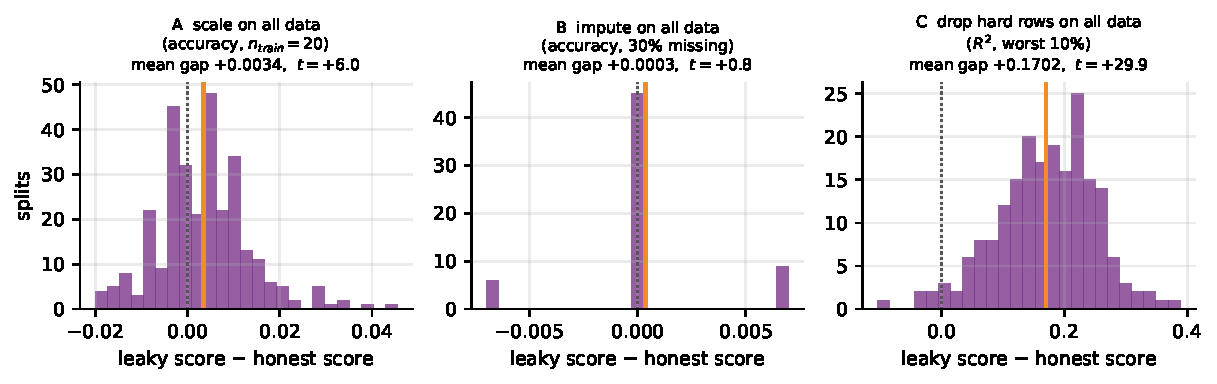
\includegraphics[width=0.96\textwidth]{leakage.pdf}
  \end{center}
  \begin{center}\small
    Each histogram is the per-split difference, leaky minus honest. Note the
    horizontal scales: $0.04$, $0.008$ and $0.4$. \textbf{Do not learn ``all
    leakage is catastrophic'' and do not learn ``leakage is overblown''. Learn
    to ask what the step learned from the test set.}
  \end{center}
\end{frame}

\begin{frame}[fragile,shrink=4]{The pipeline that cannot leak}
\begin{lstlisting}
pipe = Pipeline([
    ("impute", SimpleImputer(strategy="median", add_indicator=True)),
    ("power",  PowerTransformer(method="yeo-johnson")),
    ("scale",  StandardScaler()),
    ("model",  LogisticRegression(max_iter=5000)),
])
cross_val_score(pipe, X_with_holes, y, cv=5).mean()
\end{lstlisting}
\begin{outblk}
one Pipeline, 5-fold cross-validation, 10% of cells missing
  steps: impute -> power -> scale -> model
  cross_val_score  0.9578  +/- 0.0140
\end{outblk}
\onslide<2->
\begin{center}\small
  Every step is refitted inside every fold. The median, $\lambda$, the mean and
  the sd are all recomputed nine times, from four fifths of the data, and the
  held-out fifth is never touched.
  \textbf{There is nothing left for you to get wrong by hand --- which is the
  entire reason \texttt{Pipeline} exists.}
\end{center}
\end{frame}

% =====================================================================
\section{Summary}
\label{sec:summary}

\begin{frame}[shrink=14]{Summary --- data cleaning in twelve lines}
  \begin{enumerate}\small
    \item Deletion is exponential in the number of columns. $5\%$ of cells
      missing across $30$ features left $114$ of $569$ patients.
    \item Mean imputation preserves the mean and multiplies the variance by
      exactly $m/n$: measured $0.9486$ against $\sqrt{0.9}=0.9487$, and
      $0.5447$ against $\sqrt{0.3}=0.5477$.
    \item That shrinkage propagates: $\mathrm{corr}(\text{BMI},y)$ fell from
      $0.5865$ to $0.4538$ at $40\%$ imputed.
    \item \textbf{MCAR} bias $+0.12$, \textbf{MAR} $+1.35$, \textbf{MNAR}
      $-2.95$ kg/m$^2$. MICE fixed MAR ($+1.35 \to -0.16$) and could not fix
      MNAR ($-2.95 \to -2.58$).
    \item Under MNAR, mean imputation flipped a coefficient's sign:
      $5.60 \to -0.41$.
    \item Dropping incomplete rows cost $0.05$ of $R^2$; the choice among six
      imputers cost $0.003$. \textbf{Spend your attention accordingly.}
    \item \texttt{add\_indicator=True} was worth $+0.1675$ accuracy when the
      missingness itself carried the signal.
    \item \textbf{Thirty good readings and five stuck at $100$: the $|z|>3$
      rule flagged none of them.} The modified $z$ flagged exactly five.
    \item Masking gets worse with more contamination: caught at $z=5.38$ with
      one outlier, $3.11$ with three, never from four onwards.
    \item $|z|$ can never exceed $(n-1)/\sqrt n$, so below $n=11$ the rule
      cannot fire at all.
    \item On a skewed column the three rules flagged $6$, $65$ and $81$ rows;
      after one Yeo--Johnson, $0$, $1$ and $0$. Box--Cox took skewness
      $5.43 \to 0.06$ at $\lambda = -0.4357$.
    \item Scaling before the split was worth $+0.0034$; deleting badly-fitted
      rows before the split was worth $+0.1702$. \textbf{Use a
      \texttt{Pipeline} and neither can happen.}
  \end{enumerate}
\end{frame}

\begin{frame}[shrink=3]{Before the next lecture}
  \begin{columns}[T]
    \begin{column}{0.48\textwidth}
      \begin{block}{Read}
        \texttt{notes.pdf} --- the full variance-shrinkage derivation, the
        $(n-1)/\sqrt n$ proof, and \textbf{10 practice questions with worked
        solutions}.
      \end{block}
      \begin{block}{Do}
        Questions 2, 5 and 9. Question 5 is the three outlier rules by hand;
        question 9 is a debugging story you will meet for real.
      \end{block}
    \end{column}
    \begin{column}{0.48\textwidth}
      \begin{exampleblock}{Next: feature engineering}
        Scaling, encoding, and reducing the number of columns. Carry one thing
        across: \textbf{every one of those steps also learns a number from the
        training set.}
      \end{exampleblock}
      \begin{alertblock}{And a habit to start now}
        Before you fit anything: how many holes, why, and what does the
        histogram of each column look like?
      \end{alertblock}
    \end{column}
  \end{columns}
  \begin{center}
    \small Materials: \texttt{\AMLRepoURL}
  \end{center}
  \slidesources{\AMLUnitIVSources}
\end{frame}

\end{document}
